\documentclass[11pt, letterpaper, journal]{IEEEtran}

\usepackage[utf8]{inputenc}
\usepackage[letterpaper, margin=1.5cm]{geometry}
\usepackage{amsmath}
\usepackage{amssymb}
\usepackage{amsthm}
\usepackage[title]{appendix}
\usepackage{authblk}
\usepackage{cite}
\usepackage[font=scriptsize]{caption}
\usepackage{graphicx}
\usepackage{subcaption}
\usepackage{xcolor}
\usepackage{multicol}
\usepackage{lipsum}

% Some general setting
\graphicspath{ {./statics/} }
\captionsetup{justification=raggedright, singlelinecheck=false}


\title{Project 2: Arctic Cloud Detection}
\author[1]{Devin Ti}
\author[1]{Ryan Tang}
\affil[1]{Duke University, Statistical Science}

\date{December 6th 2022}

\begin{document}
\maketitle

\section{Introduction}
Global warming and how surface air temperatures changes has been a general scientific interest and public policy issue. In addition, many global climate studies predicted the global surface air temperature has the strongest correlation with the increase of the Arctic's atmospheric carbon dioxide level. Hence understanding how carbon dioxide changes in the Arctic is crucial to studying global warming. As the Arctic gets warmer, water vapors and changes in the distribution and proportionality of clouds can lead to further warming and spatial sensitivity, which indicates we need a systematic, accurate way of studying cloud distribution in the Arctic. However, such a study has its unique challenges. Primarily, the current algorithm not being well-suited for distinguishing clouds from ice particles because the two particles are similar in the lens of radiation measurements. MISR data offers a potential solution and introduces a sheer amount of data volume. But the currently deployed algorithm in MISR is not particularly targeted for detecting clouds over bright surfaces in polar regions. At the same time, computational constraints also limit the existing algorithm's performance. Therefore, coming up with a computationally efficient algorithm that delivers accurate detection is of the utmost importance.

MISR provides Arctic satellite images on each orbit on each path every 16 days interval. Each resulting data unit is an image concentrating on a particular, repeating Arctic location patch. Tao and other members of his team took the time to manually label the data unit with the aid of a labeling algorithm from Jet Propulsion Laboratory, which resulted in 71.5\% of conservative, expert label coverage at the pixel level for evaluating the algorithms, \{-1 = Not Cloudy, 0 = Not Sure, 1 = Cloudy\}. Furthermore, Tao's team introduced ELCM, a cloud detection algorithm based on the three expert-designed features using just if-else hard-coded rules, and utilized Quadratic Discriminant Analysis (QDA) for probabilistic prediction on top of ELCM labels that achieved astonishing results both in terms of precision and recall.

Tao's team introduced three expertly designed features through domain knowledge: CORR, SD, and NDAI. On a high level, these features were constructed through spatial convolution over a small grid under the knowledge that the aggregated radiation from multiple cameras is different between smoothed surfaces, ice and snow, and cloud. We should expect high CORR and small SD over clear or low-altitude cloud areas. NDAI provides a proxy to the visible wavelength where we should expect smaller, less volatile measures for ice and snow-covered surface than low-altitude clouds to further aid in distinguishing between the surface area from the low-altitude cloud. 

\section{Exploration}
\begin{figure*}[!h]
\centering
% \captionsetup{justification=centering}
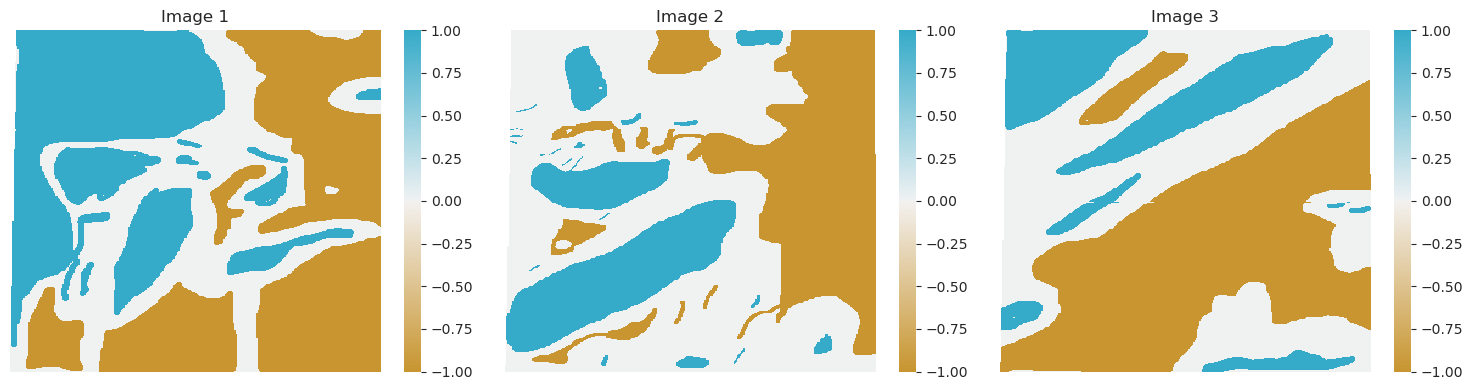
\includegraphics[width=1.0\textwidth]{1.a.png}
\caption{Three data units taken at different times at the same Arctic location. Each pixel is color coded by its respective expert label. Cloudy for blue, Brown for surface, and White for unlabeled pixels.}
\label{fig:image_labels}
\end{figure*}

\lipsum[2-4]

\section{Preparation}
\lipsum[2-4]

\section{Modeling}
\lipsum[2-4]

\section{Diagnostics}
\lipsum[2-4]

\section{Conclusion}
\lipsum[2-4]

\section{Appendix}
\lipsum[2-4]

\end{document}